%
%  untitled
%
%  Created by Asger Pedersen on 2012-01-04.
%  Copyright (c) 2012 . All rights reserved.
%
\documentclass[]{article}

% Use utf-8 encoding for foreign characters
\usepackage[utf8]{inputenc}

% Setup for fullpage use
\usepackage{fullpage}

% Uncomment some of the following if you use the features
%
% Running Headers and footers
%\usepackage{fancyhdr}

% Multipart figures
%\usepackage{subfigure}

% More symbols
%\usepackage{amsmath}
\usepackage{amssymb}
%\usepackage{latexsym}

% Surround parts of graphics with box
\usepackage{boxedminipage}

% Package for including code in the document
\usepackage{listings}

% If you want to generate a toc for each chapter (use with book)
\usepackage{minitoc}

% This is now the recommended way for checking for PDFLaTeX:
\usepackage{ifpdf}

%\newif\ifpdf
%\ifx\pdfoutput\undefined
%\pdffalse % we are not running PDFLaTeX
%\else
%\pdfoutput=1 % we are running PDFLaTeX
%\pdftrue
%\fi

\ifpdf
\usepackage[pdftex]{graphicx}
\else
\usepackage{graphicx}
\fi
\title{ Project Course: Development Studio \\ Deliverable 3: Sprint \#2}
\author{ Asger Pedersen, Kristoffer Cobley, Hari Charan \& Jesper Tved }
\setlength{\parindent}{0pt}
\setlength{\parskip}{2ex}
\linespread{1.3}

\begin{document}

\ifpdf
\DeclareGraphicsExtensions{.pdf, .jpg, .tif}
\else
\DeclareGraphicsExtensions{.eps, .jpg}
\fi

\maketitle
\setcounter{tocdepth}{1}
\tableofcontents
\newpage
\section{Sprint Material} % (fold)
\label{sec:Sprint Material}
\subsection{Version} % (fold)
\label{sub:Version}
The current state of our app has version 0.0.1. Meaning that the app is still alpha quality, with some functionality implementet, but lot of unfinished work.
% subsection Version (end)
\subsection{Source code} % (fold)
\label{sub:Source code}
We still use Git and GitHub. The source code is available at: \verb!https://github.com/mundane/ETA_analytics!, in the app folder. The other folders contains prototypes and experiments.
% subsection Source code (end)
\subsection{Sprint Explanation}
The burndown chart shows that, in spite of exams and easter holidays stalled the progress of development in the beginning of the sprint, we did manage to finish some of the tasks within the sprint time frame.
\begin{figure}[h!]
  \centering
    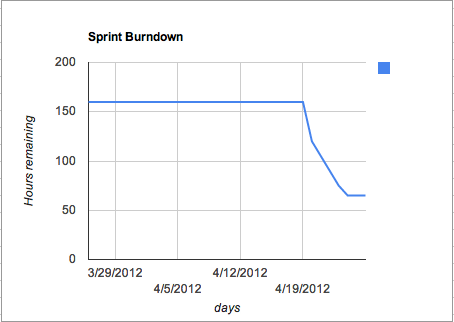
\includegraphics[width=0.8\textwidth]{images/burndown.png}
	\caption{Burndown chart for sprint \# 2. Easter holidays and exams is the reason for the steep curve.}
\end{figure}

\subsection{User Stories}
For sprint \# 2 we had the following user stories: \\
As an analytic \\
I want to make pie charts, column charts, bar charts, etc \\
So that I can make data more presentable \\

As an analytic \\
I want to make charts interactive  \\
So that I can make data more presentable \\

As an analytic \\
I want a way to show selected data from the chart \\
So that I can make data more presentable\\

As an analytic \\
I want to save data for later sessions \\
So I can continue working on datasets \\

\subsection{Tasks} % (fold)
\label{sub:Tasks}
We divided the stories up in the following tasks
% subsection Tasks (end)Tasks
\begin{itemize}
	\item Read up on the MVC model
	\item Research testing tools for Sencha
	\item Research JSLint
	\item Convert CSV format to JSON
	\item Create datagrid from JSON
	\item Make integration to Jstat in the datagrid view
	\item Create charts
\end{itemize}










% section Sprint Material (end)


\section{Sprint Retrospective} % (fold)
\label{sec:Sprint Retrospective}

% section Sprint Retrospective (end)

\section{Learning Goals} % (fold)
\label{sec:Learning Goals}

% section Learning Goals (end)
\subsection{Testing} % (fold)
\label{sub:Testing}
We used a testing tool developed for Sencha, called Siesta. Due to time restrictions, we didn't set up extensive testing, but made a simple test, to make sure that the elements of the MVC framework existed and could be reached from the app. \\
We chose Siesta, because it offers interesting testing possibilities for unit testing, such as simulating clicks and dragging of objects, which makes it easier to test user interface functionality. Other than that, the program has a lot of different built-in assertion functions, which will be useful for unit testing. When run, the program gives a visual overview of successful and failed tests, and gives an overview of where in the code an error is. The tests can be run from a GUI, which makes it easy to run the tests.
Siesta comes in two packages, where we use the free lite version. \\
We intend to use testing more intensively in the future sprints, but have not done so yet, because time was spend on other tasks, like graphing, export of graphs, and user experience elements for the app. \\
In this sprint we have not used a test-driven approach, while developing.
% subsection Testing (end)
\subsection{Static Code Analysis} % (fold)
\label{sub:Static Code Analysis}
There are not that many static code analysis tools for JavaScript. Mostly, people recommend JSlint (http://www.jslint.com/). We also looked at http://www.brics.dk/TAJS/, but we could not find any way to download it, so we had to stick with JSlint. The downside with using JSlint is that it is only for online use. Making it a cumbersome process to check a lot of code. 
Instead we used both a commmand line interface version of JSlint, via the node.js package manager and JShint, (http://www.jshint.com/) that has plugins for different text-editors. We also looked at Google's closure compiler, (https://developers.google.com/closure/), which both does static code analysis and minification of the code.\\
Futher down the line we would like to integrate static code analysis in the build process. We will most likely be using Google's closure compiler to do that. Or just use coffeescript, (http://coffeescript.org/) which compiles to JavaScript, through JSlint.\\
Using JSlint on our project in its current state did not reveal any critical bugs in our code. Mostly JSlint complains about wrong indentation

% subsection Static Code Analysis (end)

\bibliographystyle{plain}
\bibliography{}
\end{document}			